%% Reviewer supplement for the focused TORS manuscript.
%% The main paper remains main.tex/main-acmsmall.tex; this target carries the
%% extended secondary-study record and appendices without deleting evidence.
\documentclass[acmsmall,screen]{acmart}

\newif\ifmainpaper
\mainpaperfalse
\newif\ifextendedmaterial
\extendedmaterialtrue
\newif\ifincludeappendices
\includeappendicestrue

\acmJournal{TORS}
\acmYear{2026}
\setcopyright{none}
\settopmatter{printacmref=false}
\acmDOI{}
\citestyle{acmauthoryear}

\usepackage{tabularx}
\usepackage{longtable}
\usepackage{xr-hyper}
\externaldocument{main-acmsmall}
\usepackage{cleveref}
\crefname{figure}{Fig.}{Figs.}
\Crefname{figure}{Fig.}{Figs.}
\newcolumntype{Y}{>{\raggedright\arraybackslash}X}
\providecommand{\tightlist}{\setlength{\itemsep}{0pt}\setlength{\parskip}{0pt}}
\setlength{\emergencystretch}{3em}
\hyphenation{Musical-Instruments Video-Games Beauty-and-Personal-Care}
\graphicspath{{../figures/}}

\begin{document}

\title[Reviewer supplement]{Reviewer Supplement: Artifact-Gated Evaluation of a Causal FIR Module for Sequential Recommendation}
\author{[Maintainer: real author name(s) required -- TORS is single-blind]}
\affiliation{%
  \institution{[Maintainer: real institution required -- TORS is single-blind]}
  \country{[Maintainer: country]}}
\renewcommand{\shortauthors}{[Maintainer: short author list]}

\begin{abstract}
This reviewer supplement preserves the extended secondary-study record, negative
results, protocol chronology, and appendix tables omitted from the length-focused
main manuscript. It changes no verdict, claim boundary, or evidentiary status.
\end{abstract}

\maketitle

%% GENERATED from PAPER_SUBMISSION.md (pandoc) -- hand-fixed conversion; see BUILD_NOTES.md
\section{Results}\label{sec:5}

\textbf{Statistical reporting conventions.} Unless stated otherwise: the sample unit is the training seed; means are reported \ensuremath{\pm} sample standard deviation over seeds; confidence intervals are two-sided 95\% Student-t intervals with df = n\ensuremath{-}1 (n = 5 unless noted); comparisons against our own arms are seed-paired, comparisons against published numbers are point-estimate comparisons (the comparator is single-seed and unpaired); pooled tail hit-count contrasts use an unpaired two-proportion z (conservative) with the user-evaluation as the unit; p-values are uncorrected unless a correction is named --- cells labeled \emph{confirmatory} in the artifact manifest are pre-declared or \ensuremath{\ge}5-seed, \emph{exploratory} cells are single-seed or post-hoc and carry no confirmatory weight.


\subsection{Video\_Games --- multi-seed reference numbers (NOT SOTA)}\label{sec:5.1}

Our headline result (Table 1) is built on the \textbf{HSTU-style pure-PyTorch encoder} with the two added components and stacks each lever in a controlled 5-seed ablation; Table 1a reports the SASRec-family text baselines that establish protocol parity; Table 1b compares to the reported HSTU-BLaIR reference and our SM120 compatibility-port reproduction.

%% GENERATED by _bestrec_run/emit_latex_tables.py -- DO NOT EDIT BY HAND
% table key: table1
% provenance: md lines 257-265; family=hstu_tables.json:table1; check={"checked": 19, "exact": 18, "within_1ulp": 1, "allowlisted": 0, "fail": []}
\par\medskip\begingroup\small\setlength{\tabcolsep}{4pt}\renewcommand{\arraystretch}{1.12}
\noindent \textbf{Table 1: Headline component ablation --- NDCG@10 on AR2023 Video\_Games 5-core LLOO (full-catalog eval, n\_eval = 94,762; 5 seeds = 20260608\ldots20260612 unless noted; the full-model row is 6-seed 20260608\ldots20260613; one flag added per row).}\par\smallskip
\noindent
\begin{tabularx}{\linewidth}{Yrcp{0.30\linewidth}}
\toprule
Configuration & NDCG@10 & seeds & \ensuremath{\Delta} \\
\midrule
HSTU-style encoder, plain & 0.0588 & 1 & --- \\
+ TAPE-512 (sub-additive text component) & 0.0597 & 1 & +0.0009 \\
+ full bias stack (TAPE + time + text-sim + pos-rab) & 0.0637 \ensuremath{\pm} 0.0003 & 5 & +0.0049 vs plain (+8.3\%) \\
+ label smoothing \ensuremath{\varepsilon}=0.2 \citep{szegedy2016rethinking} & 0.0649 \ensuremath{\pm} 0.0003 & 5 & +0.0012 (bands non-overlapping) \\
\textbf{+ causal FIR filter K=8 (ours) \ensuremath{\rightarrow} full model} & \textbf{0.0673 \ensuremath{\pm} 0.0003} & \textbf{6} & \textbf{+0.0024 (bands non-overlapping)} \\
\emph{(single-arm)} FIR package arm (filter component; attribution open), no label smoothing & 0.0652 \ensuremath{\pm} 0.0003 & 5 & +0.0015 vs the 0.0637 stack \\
\emph{(single-arm)} ID-only (no SBERT / no text-sim / no prototypes) & \ensuremath{\approx}0.0656 \ensuremath{\pm} 0.0002 & 5 & text adds only +0.0018 (+2.7\%) overall \\
\bottomrule
\end{tabularx}
\endgroup\par\medskip


The full model is \textbf{+17.5\%} over the published SASRec baseline (0.0573, Table 1b) on the identical protocol --- but \textbf{this win is architectural, not text-driven}: the ID-only ablation already reaches \ensuremath{\approx}0.0656 (itself +14\% over published SASRec), and the entire frozen-text stack (SBERT features + text-sim bias + prototypes) adds only \textbf{+0.00178 \ensuremath{\pm} 0.00021 (5-seed, +2.7\%)} overall. The two confirmed regularizers stack near-additively on orthogonal axes (loss target vs. embedding spectrum): label smoothing alone +0.0012, causal filter alone +0.0015, combined +0.0036 over the bias stack. Per-component single-flag attribution on the HSTU-style implementation: the \textbf{time bias is the largest classical component (+0.0027)}, label smoothing +0.0013, causal filter +0.0015, while \textbf{text-similarity bias is dead weight (\ensuremath{\pm}0.0001, drop candidate)} and \textbf{TAPE is sub-additive (+0.0009)}. \emph{(The time-bias, text-sim, and TAPE single-flag figures here are the single-seed seed-20260608 DECOMP values, honestly flagged n=1 (reported inline here, not in a table). A 4-seed multi-seed cross-check --- DECOMP5, seeds 20260609--12, HSTU-style base 0.0594 --- confirms the ordering: time bias +0.0030 (largest classical component, \ensuremath{\ge} the single-seed +0.0027), pos-rab +0.0012, TAPE +0.0004, text-sim \ensuremath{-}0.00005 (dead weight confirmed). The qualitative attribution is unchanged; the only number that materially moves is TAPE, whose multi-seed single-flag lift (+0.0004) is smaller still than the single-seed +0.0009 --- further support for its demotion from a headline component.)} The causal filter's gain is robust across kernel lengths K\ensuremath{\in}\{4,8,16,50\} (k16 marginally best \& tightest, 5-seed 0.0676 \ensuremath{\pm} 0.0002; low kernel sensitivity, \S\ref{sec:5.4}). Every capacity-\emph{adding} probe we tried instead (continuous time-decay kernel, expert heads, text-distillation, dual-text, EMA, CL4SRec, James--Stein shrinkage, niche-competition loss, heat-kernel label smoothing, spectral-shrink, cue-fusion, forced ID\ensuremath{\rightarrow}text routing) was neutral or harmful --- several with a learned scalar the model itself drove to zero (the negative-result map, tabulated in Table 2, \S\ref{sec:5.5}).

%% GENERATED by _bestrec_run/emit_latex_tables.py -- DO NOT EDIT BY HAND
% table key: table1a
% provenance: md lines 281-283; family=hstu_tables.json/manifest:table1a; check={"checked": 2, "exact": 2, "within_1ulp": 0, "allowlisted": 0, "fail": []}
\par\medskip\begingroup\small\setlength{\tabcolsep}{4pt}\renewcommand{\arraystretch}{1.12}
\noindent \textbf{Table 1a: Traceable within-paper SASRec-family floor (full-catalog eval).}\par\smallskip
\noindent
\begin{tabularx}{\linewidth}{p{0.22\linewidth}rrY}
\toprule
Method & NDCG@10 & HR@10 & Notes \\
\midrule
popularity & 0.0125 & 0.0248 & trivial floor (traceable: \texttt{results\_5core\_Video\_\allowbreak Games.json}) \\
\bottomrule
\end{tabularx}
\endgroup\par\medskip


\emph{The v1-era SASRec/SBERT/BLaIR baseline rows and the observations derived from them have been REMOVED per the artifact-graph gate: their per-seed artifacts were not retained and the values are untraceable. Protocol parity is established independently by the dataset-identity statistics (exact user/item match, \ensuremath{\pm}1 interactions on every category), the frozen split hashes, and the per-category floor runs recorded in the pre-declaration results files.}

\textbf{Table 1b: Reported and locally audited HSTU-BLaIR comparator evidence} \citep[arXiv:2504.10545]{liu2025hstublair}:

The HSTU-BLaIR paper reports on AR2023 Video\_Games 5-core LLOO with identical dataset stats to ours (25,612 items / 94,762 users / 814,585 interactions). They train for \textbf{100 epochs} following Zhai et al.'s HSTU protocol. Their single-seed numbers:

%% GENERATED by _bestrec_run/emit_latex_tables.py -- DO NOT EDIT BY HAND
% table key: table1b
% provenance: md lines 287-294; family=hstu_tables.json/manifest:table1b,table1,wearec_v1; check={"checked": 19, "exact": 7, "within_1ulp": 8, "allowlisted": 4, "fail": []}
\par\medskip\begingroup\small\setlength{\tabcolsep}{4pt}\renewcommand{\arraystretch}{1.12}
\noindent
\begin{tabularx}{\linewidth}{p{0.30\linewidth}p{0.22\linewidth}rY}
\toprule
Method & NDCG@10 & HR@10 & Comparison to ours \\
\midrule
SASRec \citep[single seed, 100 epochs]{liu2025hstublair} & \textbf{0.0573} & 0.1028 & \ensuremath{-}15\% below our full model 0.0673 \ensuremath{\pm} 0.0003 \\
HSTU \citep{zhai2024hstu} & 0.0741 & 0.1315 & +10\% above our full model \\
HSTU-OpenAI (TE3L) & 0.0742 & 0.1328 & +10\% above our full model \\
\textbf{HSTU-BLaIR \citep{liu2025hstublair}} & \textbf{0.0760} & \textbf{0.1353} & \textbf{+13\% above our full model; stronger reported reference} \\
HSTU-BLaIR local SM120 compatibility port (this audit) & 0.07382 final full-eval (exported artifact; the higher best-epoch reading survives only in an unretained WSL log and is excluded from the artifact graph) & 0.13234 final & stronger than ours; not a faithful pinned-environment reproduction \\
WEARec official model/training code (8 assessment seeds; this audit) & 0.05918 {[}0.05867, 0.05969{]} & --- & \texttt{WEAREC-BELOW-EXISTING-REFERENCE}; \ensuremath{-}0.00815 {[}\ensuremath{-}0.00869, \ensuremath{-}0.00762{]} vs our six-seed 0.06734 reference under the shared evaluator \\
\bottomrule
\end{tabularx}
\endgroup\par\medskip


\textbf{Our full model (0.0673) exceeds their published SASRec (0.0573) but does not reach their HSTU (0.0741) or HSTU-BLaIR (0.0760) on Video\_Games.} Our local compatibility-port HSTU-BLaIR run reached final full-eval NDCG@10 \texttt{0.07382} (the best-epoch reading exists only in an unretained WSL log and is excluded from the artifact graph); the run is stronger than SASRec-SBERT but carries SM120/fbgemm validity caveats.

What this paper provides relative to HSTU-BLaIR:

\begin{itemize}
\tightlist
\item
  Multi-seed std (n=5 vs their n=1)
\item
  Same-protocol multi-seed text-vs-ID ablation (ID-only vs text-augmented) under matched training (the earlier 3-method encoder ablation was retired with its v1-era rows; see the manifest's RETIRED entries)
\item
  Open-source preprocessing pipeline
\item
  Compact SASRec implementation details and bug fixes
\end{itemize}

What this paper does NOT provide:

\begin{itemize}
\tightlist
\item
  A new leaderboard result; HSTU-BLaIR's reported 0.0760 remains the stronger external reference.
\item
  A faithful pinned-environment end-to-end HSTU-BLaIR reproduction. (The encoder core block is bitwise-exact against the reference research code, \S\ref{sec:3.2}, and the reference implementation's research path runs locally under data-movement shims as environment-caveated single-run regenerations, \S\ref{sec:5.6} --- but a pinned-GPU end-to-end reproduction on compatible hardware remains future work.)
\end{itemize}

\textbf{Older published baselines on different protocols} (NOT directly comparable; for context only):

%% GENERATED by _bestrec_run/emit_latex_tables.py -- DO NOT EDIT BY HAND
% table key: table_older_baselines
% provenance: md lines 291-298; family=md-only (pandoc-converted; no JSON family); check={"checked": 0, "note": "md-only table; no JSON family"}
\par\medskip\begingroup\small\setlength{\tabcolsep}{4pt}\renewcommand{\arraystretch}{1.12}
\noindent
\begin{tabularx}{\linewidth}{p{0.34\linewidth}p{0.17\linewidth}p{0.20\linewidth}Y}
\toprule
Method & NDCG@10 & Dataset & Protocol \\
\midrule
SASRec (in TIGER paper) & 0.0318 & Amazon Beauty \textbf{2014} & their 5-core (different category, different dataset year) \\
TIGER \citep{rajput2023tiger} & 0.0384 & Amazon Beauty \textbf{2014} & their 5-core \\
SASRec (in LIGER paper) & 0.02179\ensuremath{\pm}0.00023 & Amazon Beauty \textbf{2014} & their 5-core \\
LIGER (K=20, \citet{yang2024liger}) & 0.04020\ensuremath{\pm}0.00044 & Amazon Beauty \textbf{2014} & their 5-core \\
LIGER (K=N, full retrieval) & 0.04738\ensuremath{\pm}0.00151 & Amazon Beauty \textbf{2014} & their 5-core \\
Best LLM-encoder in BLaIR (\citet{hou2024blair}) Table 8 & 0.0138 & AR2023 Video\_Games & \textbf{by-timestamp 8:1:1, no k-core}, UniSRec downstream \\
\bottomrule
\end{tabularx}
\endgroup\par\medskip


\textbf{Comparability caveat}: TIGER and LIGER evaluate on the older Amazon Reviews 2014 dataset, not AR2023. The BLaIR paper does evaluate on AR2023 Video\_Games but uses a by-timestamp split (no k-core filter) and a different downstream architecture (UniSRec), producing numbers \textasciitilde3-4\ensuremath{\times} lower than our 5-core LLOO numbers. The 5-core filter removes cold users and items, which substantially eases the benchmark relative to the by-timestamp variant. We therefore do \textbf{not} claim SOTA over TIGER/LIGER/BLaIR. HSTU-BLaIR is the relevant stronger AR2023 Video\_Games 5-core reference and blocks a SASRec-SBERT SOTA claim.

\textbf{2026 semantic-ID / generative retrieval line.} Recent 2026 work reports Amazon Reviews 2023 numbers in three distinct, non-interchangeable setups. (i) \textbf{Same-statistics AR2023 5-core LLOO} (the HSTU-BLaIR protocol family we evaluate in): the concurrent preprints \textbf{SID-MLP} \citep[arXiv:2605.12617]{guo2026sidmlp} and \textbf{Latte} \citep[arXiv:2605.06331]{hou2026latte} report leave-one-out numbers on the same MI/VG dataset statistics (Latte reports MI NDCG@10 0.0331 and VG 0.0515). \textbf{GrIT} \citep[arXiv:2602.19728]{shyam2026grit} likewise reports Video\_Games numbers on matching 5-core statistics with full-item-set ranking (NDCG@10 0.0588); our 5-seed 0.0673 \ensuremath{\pm} 0.0003 is numerically higher, but we have not audited concurrent preprints' training and protocol details for full comparability, so we record this as a point-estimate observation, not a claim. (GrIT also reports same-statistics numbers for Industrial\_and\_Scientific and CDs\_and\_Vinyl --- the two categories of our pre-declared FIR-breadth campaign; we note this for literature completeness only: the FIR-breadth results are internal paired filter-vs-no-filter contrasts under their frozen wording and make no comparison against GrIT or any external number.) We cite these works for completeness of the protocol family and make \textbf{no comparative claim} against concurrent arXiv-only work; their published point estimates do not alter the comparator choice --- the published HSTU-BLaIR 0.0406 remains the strongest Musical\_Instruments reference we know of in this family, and it is the point estimate our pre-declared confirmation exceeds (\S\ref{sec:5.2}). (ii) \textbf{The SID line's own filtered universe}: \textbf{ReSID} \citep[arXiv:2602.02338]{liang2026resid} reports MI NDCG@10 = 0.0346 in its main ranking table under its own filtering; \textbf{ChronoSID} \citep[arXiv:2607.03918]{huang2026chronosid}, in its output-level MI table, reports 0.0345 for ChronoSID versus 0.0325 for its ReSID reproduction. Each uses the SID line's filtered universe (57,359 users / 23,742 items / 490,522 interactions), which differs from the 57,439 / 24,587 / \textasciitilde511,835 HSTU-BLaIR-family statistics we and the comparator share; metrics and protocols are not interchangeable across the two lines, so we discuss this line rather than claim against it. (iii) \textbf{Older Amazon-2014 protocols}: TIGER/LIGER numbers predate AR2023 and are not comparable (\S\ref{sec:2.1}, Appendix A.3). (iv) \textbf{Other AR2023-adjacent, non-interchangeable protocols}: \emph{Augment or Not?}~\citep[arXiv:2505.23053]{huang2025augment} benchmarks LLM recommenders on AR2023 Musical\_Instruments / Industrial\_and\_Scientific under 5-core leave-one-out (best listed MI NDCG@10 0.0282); \textbf{DiffuReason}~\citep[arXiv:2602.09744]{jiang2026diffureason} evaluates an AR2023 ``Video \& Games'' universe with different rating filtering and statistics (67,658 users / 25,535 items / 654,867 interactions, vs this family's 94,762 / 25,612 / \textasciitilde814,586), so its HSTU-backbone numbers are not comparable to any number in this paper --- we cite it precisely to flag that non-comparability, which also reinforces why we make no Video\_Games claims. A further candidate, \textbf{SILLM4Rec} \citep[MMAsia 2025; DOI 10.1145/3743093.3771011]{wu2025sillm4rec}, is excluded on a now-confirmed protocol distinction (full text inspected 2026-07-19): its evaluation samples 500 disjoint Video\_Games test users, caps histories at the most recent 20 items, and ranks one held-out positive against nine randomly selected negatives (its \S4.1.3--4.1.4), so its reported Video\_Games NDCG@10 of 0.6073 (its Table 1) is a ten-candidate sampled-ranking number, not comparable to any full-catalog value in this paper. Finally, three further 2026 semantic-ID works are cited for coverage and are explicitly out of scope: \textbf{UniSGR} \citep[arXiv:2607.04068]{sun2026unisgr} evaluates semantic-ID generation-plus-ranking on private industrial logs with online A/B testing, not public AR2023 LLOO; \textbf{DIGER} \citep[arXiv:2601.19711]{fu2026diger} studies differentiable semantic-ID learning; \textbf{ACERec} \citep[arXiv:2602.13573]{xia2026acerec} targets long semantic IDs across six benchmarks. Per the checked evidence none evaluates the AR2023 full-catalog LLOO protocol family on our categories, and we make no comparison against any of them.

What we \emph{can} claim:

\begin{itemize}
\tightlist
\item
  Among our HSTU-style full-catalog AR2023 5-core LLOO runs, SASRec-SBERT is a strong, simple, compact baseline --- with no priority claim for the protocol: HSTU-BLaIR published AR2023 5-core numbers before this work, and 2026 preprints report further AR2023 LLOO numbers on the same dataset statistics (the concurrent-preprint paragraph in \S\ref{sec:5.1}). It is using only 11.6M parameters and \textasciitilde10 min of training on a single consumer GPU.
\item
  Compared to a popularity floor (0.0125), our model achieves a 4.1\ensuremath{\times} improvement, indicating the model is learning meaningful sequential structure rather than just popularity.
\end{itemize}


\subsection{The causal FIR filter carries the cross-category generalization (Musical\_Instruments)}\label{sec:5.2}

The single most important robustness result for the filter is that it transfers to a \emph{second} category, and does so \emph{more strongly than label smoothing}. On Musical\_Instruments (a sparser AR2023 category), the full V2 stack reaches \textbf{NDCG@10 = 0.0413 \ensuremath{\pm} 0.0005 (5-seed)}, \textbf{+7.9\%} over a matched HSTU+TAPE base (0.0383 \ensuremath{\pm} 0.0004) and \textbf{+57\%} over a plain ID-only SASRec (0.0264). A controlled single-lever isolation (best-by-val, vs the MI SBERT+TAPE base 0.0383, 4\ensuremath{\times}e20-seed) dissociates the two confirmed regularizers:

%% GENERATED by _bestrec_run/emit_latex_tables.py -- DO NOT EDIT BY HAND
% table key: table1c
% provenance: md lines 301-306; family=hstu_tables.json:table1c; check={"checked": 9, "exact": 7, "within_1ulp": 2, "allowlisted": 0, "fail": []}
\par\medskip\begingroup\small\setlength{\tabcolsep}{4pt}\renewcommand{\arraystretch}{1.12}
\noindent \textbf{Table 1c: Musical\_Instruments per-lever isolation (NDCG@10, best-by-val, vs MI SBERT+TAPE base; shares are of the 5-seed V2 combined lift +0.0032).}\par\smallskip
\noindent
\begin{tabularx}{\linewidth}{Yrrr}
\toprule
Configuration & NDCG@10 & \ensuremath{\Delta} vs base & share of combined lift \\
\midrule
MI SBERT+TAPE base (4\ensuremath{\times}e20-seed) & 0.0383 & --- & --- \\
+ label smoothing only (5-seed) & 0.0391 \ensuremath{\pm} 0.0001 & +0.0008 & 26\% \\
\textbf{+ causal filter only (k16, 5-seed)} & \textbf{0.0408} & \textbf{+0.0025} & \textbf{77\%} \\
+ both = V2 (k16, 5-seed) & 0.0415 & +0.0032 & 100\% \\
\bottomrule
\end{tabularx}
\endgroup\par\medskip


(Recomputed best-by-val from the released per-seed artifacts. Against the headline 5-seed V2 stack the filter's share is 77\% (k16) / 82\% (k8). LS-only is the 5-seed family \texttt{results\_MI\_lsonly\_seed\{08–12\}} (0.03914 \ensuremath{\pm} 0.00013); base is the four e20 seeds 20260609--12.)

\textbf{The causal filter contributes \ensuremath{\approx}3\ensuremath{\times} what label smoothing does on the second category, and \ensuremath{\approx}80\% of the combined lift (77\% vs the k16 stack, 82\% vs the k8 headline stack)} --- i.e. the filter generalizes cross-category while label smoothing is largely Video\_Games-specific. The filter's kernel-robustness also generalizes (MI k8 0.0413 \ensuremath{\pm} 0.0005 \ensuremath{\approx} k16 0.0415 \ensuremath{\pm} 0.0002). This locks the causal FIR filter as the paper's primary methodological anchor: a leak-free, simple, parameter-cheap operation supplying an explicit local temporal bias that the baseline does not learn as reliably in our low-capacity setting --- now confirmed on four categories: the two development categories plus the pre-declared breadth campaign below.

\textbf{Pre-declared breadth (two further categories).} Under \texttt{PREREG\_FIR\_BREADTH.md} (committed before any run; fresh never-inspected seeds 20260713--17; mechanical adjudication in \texttt{FIR\_BREADTH\_RESULTS.md}), the filter was transplanted with \textbf{zero per-category tuning} and tested as a paired 5-seed filter-vs-no-filter contrast --- an internal contrast with no comparator involved --- on two categories never used in its development. \textbf{Both confirmed}: Industrial\_and\_Scientific paired \ensuremath{\Delta} = \textbf{+0.0024 \ensuremath{\pm} 0.0005} (95\% CI {[}+0.0018, +0.0030{]}, 5/5 seeds positive) and CDs\_and\_Vinyl paired \ensuremath{\Delta} = \textbf{+0.0057 \ensuremath{\pm} 0.0006} (95\% CI {[}+0.0049, +0.0064{]}, 5/5 seeds positive). Per the frozen claim wording, each result is exactly this: \emph{the causal FIR filter's paired 5-seed improvement on that category is positive with a 95\% CI excluding zero} --- nothing broader, no SOTA language, no comparator statement. The filter is thus multi-seed-confirmed on \textbf{four categories}, two of them under this pre-declared breadth campaign.

\textbf{Comparator ablations (audit-requested).} Each arm targets one named design element of the filter (with the disclosed caveat that the singular headline initialization means these arms also alter the optimization path, \S
ef{sec:3}) on the same 5-seed MI stack: freezing the kernel at a causal moving average (learnable gate retained) recovers only +0.00133 of the filter's +0.00225 gain over the no-filter baseline (0.04046 \ensuremath{\pm} 0.00022 vs 0.04138 \ensuremath{\pm} 0.00053; non-overlapping bands) --- the learned kernel shape, not generic smoothing, carries the effect. Freezing the gate at 1 (delta-initialized kernel) matches the full filter (0.04127 \ensuremath{\pm} 0.00046), so the zero-init gate comparison is confounded by the singular-initialization bootstrap (\S
ef{sec:3} disclosure) and is not a clean single-factor attribution.

\textbf{Pre-declared confirmation vs the published per-category reference.} The seeds above (20260608--17) are \emph{exploratory}: kernel choice, epoch budget, and the decision to compare against the published Musical\_Instruments HSTU-BLaIR number (0.0406; \citealp[Table 2]{liu2025hstublair}) were all made while inspecting them. To make the comparison selection-free, we froze a version-controlled pre-declared protocol (\texttt{SOTA\_CONFIRM\_PREREG\_V2.md}, committed to version control before any confirmation run: exact config and commands, data SHA256s, decision rule, claim wording) and ran \textbf{five pre-specified never-inspected seeds (20260618--22) under each of the two kernels --- ten arm-runs} with per-run provenance manifests (command, git commit + clean-tree flag, environment, data hashes) and per-user record sidecars. Result: \textbf{K=16 fresh 5-seed 0.04152 \ensuremath{\pm} 0.00045 (95\% CI lower bound 0.04096) and K=8 0.04120 \ensuremath{\pm} 0.00030 (CI-LB 0.04083) --- both CI lower bounds above the published 0.0406, 10/10 seeds above.} The supported claim is exactly this: \emph{fresh multi-seed means and seed-level confidence intervals exceed the published HSTU-BLaIR point estimate on this category under our reproduced protocol (parity evidence: users/items match the paper exactly; interactions differ by one --- see \texttt{SOTA\_CONFIRM\_PREREG\_V2\_ERRATA.md} E1; our plain SASRec floor is} below \emph{their published SASRec, ruling out an easier split).} The comparator is single-seed; our post-hoc local regeneration of it (\S\ref{sec:5.6} --- the reference implementation's research path under data-movement shims, unpinned environment) regenerates the published value at its best full-eval epoch (0.0406; final epoch 0.0391) but is itself a single environment-caveated run, so no paired or distributional superiority is claimed, and this remains a per-category result --- Video\_Games is explicitly not claimed (\S\ref{sec:5.1}). The first execution of this confirmation was voided by its own provenance tripwire (a concurrent documentation edit dirtied the tracked tree mid-campaign) and re-executed in full under a clean tree; both executions agree per-seed to \ensuremath{\pm}0.0003 (\texttt{SOTA\_CONFIRM\_V2\_RESULTS.md}). One protocol deviation is disclosed rather than claimed away: the gated runs executed at a documentation-only descendant commit of the pre-declaration's introducing commit (the pre-declared commit-equality rule was not literally satisfied); code identity across the two commits is demonstrated by empty protocol-file diffs and, in the from-scratch rebuild, by code hashes embedded in each run manifest (\texttt{SOTA\_CONFIRM\_PREREG\_V2\_ERRATA.md}, E3).

%% GENERATED by _bestrec_run/emit_latex_tables.py -- DO NOT EDIT BY HAND
% table key: tableV2conf
% provenance: hstu_tables.json family 'tableV2conf' (regenerated by build_hstu_tables.py --submission)
\par\medskip\begingroup\small\setlength{\tabcolsep}{4pt}\renewcommand{\arraystretch}{1.12}
\noindent \textbf{\S\ref{sec:5.2} (regenerated): pre-declared dual-kernel V2 confirmation (SOTACONF\_V2, fresh seeds 20260618--22, EXEC2 gated artifacts, n\_eval=57,439).}\par\smallskip
\noindent
\begin{tabularx}{\linewidth}{lccY}
\toprule
kernel & fresh 5-seed NDCG@10 & 95\% CI lower bound & vs published 0.0406 \\
\midrule
K=16 & 0.04152 \ensuremath{\pm} 0.00045 & 0.04096 & ABOVE \\
K=8 & 0.04120 \ensuremath{\pm} 0.00030 & 0.04083 & ABOVE \\
\bottomrule
\end{tabularx}
\par\smallskip\noindent{\footnotesize Fresh seeds above 0.0406: 10/10. EXEC1\ensuremath{\leftrightarrow}EXEC2 max per-seed \textbar \ensuremath{\Delta}\textbar{} = 0.000057 (\textless{} 0.0003). Clean rebuild (rebuild\_v2/): K=16 CI-LB 0.04092, K=8 CI-LB 0.04084 --- dual gate PASS.\par}
\endgroup\par\medskip


\textbf{Office\_Products V1 (the original second-category attempt) --- descriptive only; superseded by the counted V3 campaign below.} Office\_Products numerically exceeded the published HSTU-BLaIR point estimate under the frozen MI configuration, but the pre-declared SASRec floor check failed because our local SASRec floor was substantially above the published SASRec reference. We therefore treat the V1 Office campaign as descriptive evidence, not as a passed confirmatory category (the separately pre-declared V3 campaign later passed and is counted, \S\ref{sec:5.2}). The floor anomaly has since been resolved mechanistically --- the reference implementation's own SASRec, run locally on its own pipeline (\S\ref{sec:5.6}), lands +13.9\% above its published row, while a completed run of their Office HSTU-BLaIR configuration regenerates its published row (+1.6\%; \S\ref{sec:5.6}) --- the conservatism is a property of the published Office SASRec row specifically. The VOID is retained on procedural grounds (the pre-declared floor check failed as written); full detail, decomposition, and disclosures in Appendix A.0.

\textbf{Office\_Products V3 (redesigned pre-declaration) --- PASSED.} Under \texttt{PREREG\_OFFICE\_V3.md} (committed before any run; fresh never-inspected seeds 20260728--32; gate: each arm's fresh 5-seed 95\% CI lower bound must exceed the \textbf{environment-matched local regeneration of the comparator} --- best full-eval 0.0279, itself above the published 0.0271 --- with \ensuremath{\ge}4/5 seeds individually above), \textbf{both kernel arms passed}: K=16 fresh 5-seed \textbf{0.03047 \ensuremath{\pm} 0.00011 (CI-LB 0.03033)} and K=8 \textbf{0.03029 \ensuremath{\pm} 0.00005 (CI-LB 0.03024)}, 10/10 seeds above both references; dataset identity, reference-artifact hashes, and per-run provenance verified mechanically (\texttt{OFFICE\_V3\_RESULTS.md}). Per the frozen claim wording: \emph{a per-category point-estimate comparison against the published 0.0271 and its environment-matched single-run local regeneration 0.0279; no paired or distributional superiority is claimed; this is not SOTA on Office\_Products, not SOTA on Amazon Reviews 2023, and not a general-SOTA claim of any kind.} The V1 VOID above stands unchanged as its own record (Appendix A.0).


\subsection{A dataset-conditional long-tail pattern for text-augmented recommendation}\label{sec:5.3}

Beyond \emph{whether} text helps overall (modestly: +2.7\% on Video\_Games, \S\ref{sec:5.1}), we ask \emph{where} it helps. \texttt{evaluate()} reports \texttt{by\_popularity} NDCG@10 over train-frequency terciles \{tail, mid, head\} (bucketed by TRAIN frequency only --- leak-free), and we compare the full text stack against an ID-only ablation on the \textbf{same split and seeds}, the controlled \texttt{text\ \ensuremath{-}\ ID} tail contrast. The cold-start intuition --- text should rescue rare items where ID embeddings are starved --- holds on \emph{one} of three datasets, and the difference is principled and significant.

%% GENERATED by _bestrec_run/emit_latex_tables.py -- DO NOT EDIT BY HAND
% table key: table1d
% provenance: md lines 318-322; family=hstu_tables.json:table1d; check={"checked": 8, "exact": 7, "within_1ulp": 1, "allowlisted": 0, "fail": []}
\par\medskip\begingroup\small\setlength{\tabcolsep}{4pt}\renewcommand{\arraystretch}{1.12}
\noindent \textbf{Table 1d: text \ensuremath{-} ID tail-tercile NDCG@10 contrast (paired, per-seed; the dataset-conditional pattern).}\par\smallskip
\noindent
\begin{tabularx}{\linewidth}{p{0.22\linewidth}p{0.10\linewidth}Ycp{0.14\linewidth}}
\toprule
dataset & catalog density & tail \ensuremath{\Delta} NDCG@10 (5-seed) & seeds positive & verdict \\
\midrule
\textbf{Musical\_Instruments} & sparse & \textbf{+0.000335 \ensuremath{\pm} 0.000195}, 95\% CI {[}+0.00009, +0.00058{]} \textbf{excl 0} & \textbf{5/5} & \textbf{text WINS the tail} \\
\textbf{Video\_Games} & dense & \ensuremath{-}0.000148 \ensuremath{\pm} 0.000179 & 2/5 & \textbf{powered NULL} \\
\textbf{Beauty\_and\_\allowbreak PC} & dense & \ensuremath{-}0.0000078 (3-seed, sample-sd 0.000020) & 1/3 & NULL \\
\bottomrule
\end{tabularx}
\endgroup\par\medskip


Three points make this a defensible empirical \emph{pattern} rather than a lucky bucketing:

\begin{enumerate}
\def\labelenumi{\arabic{enumi}.}
\tightlist
\item
  \textbf{The MI tail win is real and replicates on a rank-free metric.} Tail HR \ensuremath{\Delta} = +0.00109 \ensuremath{\pm} 0.00065, 5/5 positive (\ensuremath{\approx}29.6 vs 20.0 hits/seed); all terciles are 5/5-positive. We are honest about scale: text's \emph{largest absolute} lift is at the head (+0.00527 on MI), and the tail win is a large \emph{relative} gain (+27.6\%) on a tiny (\textasciitilde30-hit/seed) base --- we always report relative, absolute, and hit-count together.
\item
  \textbf{The VG null is a \emph{powered} null, not an underpowered failure to reject} --- the standard reviewer objection to a null. VG tail \ensuremath{\Delta} = \ensuremath{-}0.000148 \ensuremath{\pm} 0.000179 (SE 0.000080); the minimum detectable effect (paired t, 80\% power, n=5) is \textbf{0.000246 \textless{} MI's native effect 0.000335}, so VG had \textgreater80\% power to see an MI-sized effect and saw none. A \textbf{TOST equivalence test} against MI's \ensuremath{\pm}0.000335 margin gives 90\% CI {[}\ensuremath{-}0.000319, +0.000023{]} \ensuremath{\subset} \ensuremath{\pm}0.000335 \ensuremath{\Rightarrow} VG's tail text-benefit is \textbf{statistically equivalent to zero} within the magnitude that matters. We state the VG/Beauty tail results as positive equivalence claims.
\item
  \textbf{The cross-dataset difference is itself significant.} Welch two-sample contrast of the per-seed paired tail \ensuremath{\Delta}: MI \ensuremath{-} VG = +0.000484, \textbf{t = 4.09, df \ensuremath{\approx} 7.9, p \ensuremath{\approx} 0.004 (two-sided)}. The pattern (sparse-catalog text wins the tail; dense-catalog text does not) is a real between-dataset effect. A companion \textbf{regime-migration} finding: text's winning tercile slides \textbf{tail \ensuremath{\rightarrow} mid \ensuremath{\rightarrow} head as catalogs densify} (MI sparse \ensuremath{\rightarrow} VG \ensuremath{\rightarrow} Beauty dense). The tail pattern and its two-axis mechanism decomposition are summarized in \textbf{\cref{fig:tail_law_mechanism}} (\texttt{figures/fig\_tail\_law\_mechanism}): panel (A) this dataset-conditional tail pattern, panel (B) the interaction-density titration double result (\S\ref{sec:5.4}), and panel (C) the connectivity-vs-count two-axis decomposition (\S\ref{sec:5.4.1}--\S\ref{sec:5.4.2}).
\end{enumerate}

%% round-7: Fig. 1 embedded (md image line; the md's duplicate italic caption line collapses into this \caption)

\begin{quote}
\textbf{Provenance/honesty:} all numbers are best-by-val paired text\ensuremath{-}ID from the released \texttt{results\_\allowbreak USERTITR\_\allowbreak\{text,idonly\}\_\allowbreak rho0\{66,50,40\}\_\allowbreak s08\ldots{}\allowbreak s12\_\allowbreak VG.json} (5 seeds each rung, n\_eval=94,762 + tail\_n=10,900 frozen at full density across every rung/seed/arm --- verified, no eval drift). The lower rungs \ensuremath{\rho_{\mathrm{user}}} 0.50/0.40 are \textbf{5-seed} (previously single-seed); the down-limb 5-seed fill \textbf{refuted} the single-seed non-monotonicity (\ensuremath{\rho_{\mathrm{user}}}=0.50 = +0.000236, 4/5 positive --- no decline; \ensuremath{\rho_{\mathrm{user}}}=0.40 = \ensuremath{-}0.001545, 1/5, a TEXT-arm floor collapse), per the floor-artifact decision rule above. The tail base is small (\textasciitilde50 hits/seed on 10,900 tail users); we report relative, absolute, and the per-seed sign count together. As in \S\ref{sec:5.4} we claim a level-dissociation (the slope-difference is n.s. at these seed counts --- level-contrast-only (the interaction test itself is not significant)).
\end{quote}


\subsection{Systematic negative-result map}\label{sec:5.5}

A central empirical finding of this work is \textbf{asymmetric}: the only levers that moved test NDCG@10 were \emph{capacity-restricting} (label smoothing, the causal FIR filter) or classical inductive biases already in Table 1 (the time bias); \textbf{every capacity-\emph{adding} probe we tried was neutral or harmful.} We document the full set here as a first-class result --- negatives are part of the contribution, and several are \emph{interpretable} negatives in which a learnable scalar, free to engage the mechanism, was driven by the optimizer to (or past) zero. This is the evidence that the in-environment ceiling is not for want of trying these mechanisms; the residual gap to the published HSTU-BLaIR 0.0760 could not be isolated (the pinned reference environment is not installable here, and the shimmed local execution of \S\ref{sec:5.6} did not include the Video\_Games configuration); what the probe set shows is that it is not explained by any of the modeling axes we could test.

All entries are best-by-val test NDCG@10, full-catalog eval (n\_eval = 94,762 on Video\_Games), on the same fixed protocol. \ensuremath{\Delta} is versus the stated base; for the three learnable-scalar probes (W1/X1/Y1) we report the absolute single-seed test next to its base band, since the headline test is statistically indistinguishable from the base and the \emph{learned scalar} is the load-bearing readout. Several rows are single-seed --- sufficient for a negative-result map (a probe that fails to clear its base on one seed, or whose own learned scalar switches it off, does not warrant five seeds).

\textbf{Unequal power, stated plainly.} The probes in Table 2 do \emph{not} carry equal evidential weight: most rows are single-seed exploratory probes, while a few were run at full multi-seed power. Only the multi-seed, pre-declared negatives --- the conn-gate five-seed paired confirmation and the titration nulls of \S\ref{sec:5.3}--\S\ref{sec:5.4} (the powered VG/Beauty tail nulls and the 5-seed-locked ladder rungs) --- carry confirmatory weight. The remaining rows are exploratory documentation of the search space, recorded for completeness and interpretability, not powered hypothesis tests. Full per-probe seed counts are given in the table's n column.

\newpage
%% GENERATED by _bestrec_run/emit_latex_tables.py -- DO NOT EDIT BY HAND
% table key: table2
% provenance: md lines 440-461; family=hstu_tables.json:table2; check={"checked": 33, "exact": 17, "within_1ulp": 13, "allowlisted": 3, "fail": []}
\par\medskip\begingroup\scriptsize\setlength{\tabcolsep}{4pt}\renewcommand{\arraystretch}{1.12}
\noindent \textbf{Table 2: Systematic negative-result map --- capacity-adding / alternative-mechanism probes, all neutral or harmful.} (Mechanism class: where the lever acts. ``Learned scalar \ensuremath{\rightarrow} 0?'' = did a free learnable gate/temperature/intensity collapse the mechanism. n = seed count. \textbf{Note: probes are not equally powered} --- most rows are single-seed exploratory probes; only the multi-seed pre-declared negatives carry confirmatory weight, per the paragraph above.)\par\smallskip
\noindent
\begin{tabularx}{\linewidth}{p{0.155\linewidth}p{0.13\linewidth}p{0.11\linewidth}p{0.16\linewidth}p{0.10\linewidth}Y}
\toprule
Lever & Mechanism class & Base (NDCG@10) & \ensuremath{\Delta} NDCG@10 (n) & Learned scalar \ensuremath{\rightarrow} 0? & Verdict \\
\midrule
c3 continuous time-decay attention kernel & attention re-weighting (capacity-add) & SBERT stack \ensuremath{\approx}0.0639 & \textbf{\ensuremath{-}0.0150} (1; test 0.0489 at record val 0.0725) & n/a & Rejected --- actively harmful; the largest validation--test divergence in the corpus \\
Sampled softmax (K=512 negatives) & loss approximation & full-softmax stack & \ensuremath{-}0.0026 (1) & n/a & Rejected --- undertrains full-catalog ranking \\
Dual text encoder (SBERT \ensuremath{\oplus} BLaIR) & text encoder & SBERT stack & \ensuremath{-}0.0014 (1) & n/a & Rejected --- the text encoder is not the gap \\
BLaIR text encoder (swap) & text encoder & SBERT stack & \ensuremath{-}0.0013 (1) & n/a & Rejected --- encoder axis fully swept \\
GD1 spectral-shrink prior & representation regularizer & V2 0.0673 & \ensuremath{-}0.003 (1) & shrink \ensuremath{\rightarrow} 0 & Rejected --- BBP irreducibility figure (\cref{fig:bbp_irreducibility}) retained \\
n\_heads = 4 & architecture (capacity-add) & HSTU-style stack & \ensuremath{-}0.0005 (1) & n/a & Rejected --- ties 2-head even at the published dv=dqk=16 spec \\
CL4SRec self-supervision & SSL auxiliary loss & SBERT stack & \ensuremath{-}0.0005 (1) & n/a & Rejected --- early-epoch only \\
c1 prototype-routed expert heads & capacity-add & SBERT stack & \ensuremath{-}0.0004 (1) & n/a & Rejected --- redundant with TAPE \\
c2 text-distillation aux loss & auxiliary loss & SBERT stack & \ensuremath{-}0.0004 (1) & n/a & Rejected --- redundant with the additive text path \\
text-init / text warm-start & embedding initialization & SBERT stack & \ensuremath{-}0.0003 (1) & n/a & Rejected --- redundant with the additive text path \\
EMA / SWA weight averaging & weight-space regularizer & SBERT stack & +0.0001 (1) & n/a & Rejected --- val-high/test-flat; does not repair the structural gap \\
text-sim bias & attention bias & HSTU-style stack & \ensuremath{\pm}0.0001 (4) & n/a & NEUTRAL --- dead weight, drop candidate \\
W1 niche-share fitness-sharing penalty & inter-item loss penalty & U2/LS0.2 0.0649\ensuremath{\pm}0.0002 & 0.0652 (1), within band & \textbf{\ensuremath{\beta} = \ensuremath{-}7.42} (sign-flipped: boosts, not penalizes, crowded niches) & Rejected --- refutes the anti-crowding remedy \\
X1 frequency-adaptive James--Stein shrinkage & representation regularizer & V2 0.0674\ensuremath{\pm}0.0003 & 0.0673 (1), within band & \textbf{c \ensuremath{\approx} 0} (\ensuremath{\lambda}\_max \ensuremath{\approx} 0.004) \ensuremath{\rightarrow} off & Rejected --- model voted shrinkage off \\
Y1 heat-kernel/manifold label smoothing & loss-target reshaping & V2 0.0674\ensuremath{\pm}0.0003 & 0.06653 (1), \ensuremath{\le} band & \textbf{T \ensuremath{\rightarrow} 0.00061} (\textless{} init) \ensuremath{\rightarrow} delta target & Rejected --- text-manifold geometry voted off \\
Z1 forced ID\ensuremath{\rightarrow}text routing & representation routing & V2 & tail \ensuremath{-}75\% (globally dead) & forced gate & Rejected --- globally harmful \\
CF1 cue-fusion gate & representation fusion & V2 / MI & flat/dead (both datasets) & gate \ensuremath{\rightarrow} 0 & Rejected --- new-lever search closed \\
conn-gate connectivity-gated cold-start ID\ensuremath{\leftrightarrow}text fusion & representation fusion/routing & V2 text stack, MI & \textbf{tail} \ensuremath{\Delta} +0.0001 \ensuremath{\pm} 0.0003, paired 95\% CI {[}\ensuremath{-}0.00025, +0.00045{]} (5); overall flat & \textbf{\ensuremath{\alpha} \ensuremath{\rightarrow} 0.0011 \textless{} init 0.0025} (voted off) & Rejected --- operationalizes the intervention-supported connectivity tail mechanism, but is not actionable (CI includes 0) \\
max\_seq\_len 200 / seq \textgreater{} 50 & sequence length & SBERT stack & \textasciitilde0 (1) & n/a & Rejected --- sequences short post-5-core \\
cosine scoring & scoring function & winning op-point & \ensuremath{\le} 0 (1) & n/a & Rejected --- dot-product better at the op-point \\
\bottomrule
\end{tabularx}
\endgroup\par\medskip


The pattern is consistent and is itself the finding: across loss-side (W1, Y1, sampled-softmax), embedding-side (X1, GD1, text-init), attention-side (c3, n\_heads, text-sim), encoder-side (BLaIR, dual-text), and auxiliary-objective (c1, c2, CL4SRec, EMA) axes, no capacity-adding mechanism produced a multi-seed test gain, and three free scalars (W1's \ensuremath{\beta}, X1's c, Y1's T) were each switched off --- or, for W1, reversed --- by the optimizer. Only anti-overconfidence regularizers (label smoothing) and the restricted causal-filter inductive bias (Table 1) transferred. This both bounds the in-environment ceiling and motivates the spectral-irreducibility analysis of \S\ref{sec:5.4.2} (\cref{fig:bbp_irreducibility}): no representation-side lever can rescue the dense-catalog tail. The conn-gate row deserves separate emphasis: it is the only entry tested at full five-seed power and the only one that directly operationalizes \emph{this paper's own intervention-supported tail mechanism} --- collaborative connectivity as the binding tail resource (\S\ref{sec:5.4.2}). A single seed showed a +0.00053 tail lift, but the pre-declared five-seed seed-paired confirmation collapsed to +0.0001 \ensuremath{\pm} 0.0003 (95\% CI {[}\ensuremath{-}0.00025, +0.00045{]}, includes zero), and the free gate scalar \ensuremath{\alpha} was driven \emph{below} its initialization (voted off). This is the cleanest illustration of the paper's central distinction: a mechanism can be \emph{supported as a driver} of the tail advantage by controlled thinning interventions (the matched-R1 paired level contrast (no interaction-test support)) yet not be \emph{actionable} through a learnable cold-start gate --- the connectivity signal the model needs is already latent in the frozen text features, leaving no residual for an explicit gate to exploit.


\subsection{Executing the reference implementation locally (post-hoc comparator regeneration)}\label{sec:5.6}

Late in this work we succeeded in running the \textbf{reference implementation itself} --- the HSTU-BLaIR repository at its released commit, unmodified (clean git tree): its preprocessing, its gin configurations, its trainer, and its eval protocol --- end-to-end on our hardware. The pinned environment (torch 2.2.2 / fbgemm\_gpu 0.6.0) remains uninstallable here (no sm\_120 kernel images, no Windows wheels); what makes execution possible under our unpinned torch 2.11 environment is that the repository's research path uses exactly \textbf{three} \texttt{fbgemm} operators, all pure data movement (\texttt{asynchronous\_complete\_cumsum}, \texttt{jagged\_to\_padded\_dense}, \texttt{dense\_to\_jagged}), which we re-implement in plain PyTorch with self-tested forward/gradient parity, plus a world-size-1 identity DDP wrapper and logging/data-acquisition patches (full shim inventory, per-run provenance, and artifacts: \texttt{THEIRS\_ON\_OURS\_REPORT.md}). No model math is touched --- the layer norms, fused projections, SiLU pointwise attention, biases, loss, and scoring all execute in the reference repository's own unmodified lines, consistent with the core-block parity evidence of \S\ref{sec:3.2}. Their own preprocessing pipeline ran with its dataset-size assertions left active and \textbf{passing} on both corpora (Musical\_Instruments: 24,587 items / 57,439 users; Office\_Products: 77,551 items / 223,308 users --- the comparator paper's exact statistics).

Two single-run results (their configurations as shipped, 101 epochs; our RTX 5060 Ti):

%% GENERATED by _bestrec_run/emit_latex_tables.py -- DO NOT EDIT BY HAND
% table key: table56_theirs
% provenance: md lines 425-431; family=hstu_results_manifest.json:theirs_on_ours(+published constants); check={"checked": 15, "exact": 15, "within_1ulp": 0, "allowlisted": 0, "fail": []}
\par\medskip\begingroup\small\setlength{\tabcolsep}{4pt}\renewcommand{\arraystretch}{1.12}
\noindent
\begin{tabularx}{\linewidth}{Yccc}
\toprule
run (their code, their data, their eval) & published & local, final epoch & local, best full eval \\
\midrule
\textbf{MI HSTU-BLaIR} --- NDCG@10 & 0.0406 & 0.0391 & \textbf{0.0406} (epoch 35 --- exact) \\
MI HSTU-BLaIR --- HR@10 & 0.0733 & 0.0716 & 0.0743 \\
MI HSTU-BLaIR --- MRR & 0.0371 & 0.0355 & 0.0369 \\
\textbf{Office SASRec} --- NDCG@10 & 0.0153 & \textbf{0.0174} (+13.9\%) & 0.0177 \\
\textbf{Office HSTU-BLaIR} --- NDCG@10 & 0.0271 & 0.0275 (+1.6\%) & 0.0279 \\
\bottomrule
\end{tabularx}
\endgroup\par\medskip


\textbf{The Musical\_Instruments comparator regenerates locally.} The final-epoch full-corpus eval lands within 2.3--4.3\% of every published metric above, and the best full-eval epoch hits the published NDCG@10 exactly; the run oscillates in a 0.0384--0.0406 band from roughly epoch 30 onward (the comparator's own README notes run-to-run variability). The published 0.0406 that \S\ref{sec:5.2}'s pre-declared confirmation is measured against is therefore no longer only a transcribed constant: a local run of the generating code regenerates it under the unpinned shimmed research path, and our pre-declared CI lower bounds (0.04096 / 0.04083) sit above both its best (0.0406) and final (0.0391) local readings. \textbf{The Office\_Products floor anomaly resolves}: their own SASRec configuration lands +13.9\% above its published row here, crossing the published value at epoch 20 of 101 and never re-entering --- which, combined with our floor run, decomposes the +44\% floor-check failure entirely into published-row conservatism and baseline-strength protocol differences, leaving nothing attributable to our split or eval (resolution in Appendix A.0; the VOID is deliberately retained).

\textbf{Caveats (why these are regenerations, not reproductions).} Single runs (the reference code seeds only Python's \texttt{random}, so even in place it is not run-to-run deterministic); an unpinned environment (torch 2.11 vs pinned 2.2.2, transformers 5.7 vs 4.51, different cuBLAS/TF32 kernel versions); a different GPU than the comparator used; and the shims themselves --- though the shim risk has since been closed on CPU: under the pinned torch 2.2.2 itself, the real \texttt{fbgemm-gpu(-cpu)==0.6.0} operators match our shims \textbf{bit-exactly (max abs diff 0.0, forward and gradient)} on every input the pinned binary accepts, the reference block under \{pinned torch + real fbgemm\} vs \{pinned torch + shims\} is bit-exact at every stage, and the remaining torch 2.2.2\ensuremath{\rightarrow}2.11 block-level numerics drift is bounded at \textbf{4.8\ensuremath{\times}10\ensuremath{^{-7}} per stage / 2.4\ensuremath{\times}10\ensuremath{^{-7}} end-to-end}, with negative controls confirming the harness detects 1-ulp perturbations (\texttt{PINNED\_ENV\_PARITY\_REPORT.md}); the pinned stack's \emph{GPU} (cu121) kernel numerics remain the one locally untestable component. We therefore cite these as \textbf{environment-caveated single-run regenerations} and change no claim wording on their basis: \S\ref{sec:5.2}'s claim remains a point-estimate comparison against the published number.



	extbf{Retraction (2026-07-19).} The earlier spectral-irreducibility argument (a Baik--Ben Arous--P'ech'e / Marchenko--Pastur figure and a Gavish--Donoho effective-rank normalization) is withdrawn: the computation read only train frequencies --- never the embedding table or its spectrum --- its plotted quantity is a spiked-model overlap rather than a measured direction fraction, and the reported effective rank was produced by the GD1 truncation intervention itself (24 in one run, 22 in a repeat; the tabulated 23 matches no released artifact). The figure, the d\_eff normalization, and every ``no representation-side lever can rescue the tail'' conclusion are retracted pending a prospectively specified analysis of untreated checkpoints under a justified noise model. The related thinning-intervention findings are conditional patterns under two bundled interventions: no double dissociation is claimed (the interaction test is not significant), user-thinning is not a connectivity-only manipulation, and all model seeds share one fixed intervention draw.
\appendix
%% GENERATED from PAPER_SUBMISSION.md (pandoc) -- hand-fixed conversion; see BUILD_NOTES.md
\section*{Appendix A.0 --- Office\_Products: descriptive evidence (VOID under its pre-registration)}

\textbf{Second-category pre-registered confirmation: Office\_Products.} To test whether the per-category result generalizes, we froze a second pre-registration (\texttt{SOTA\_CONFIRM\_\allowbreak PREREG\_\allowbreak OFFICE.md}, committed before the raw data finished downloading --- before any Office statistic was knowable) with the config carried over from Musical\_Instruments \textbf{unchanged (zero category-specific tuning)} and fresh seeds 20260623--27. Dataset parity is exact (items 77,551 and users 223,308 match the comparator paper exactly; interactions differ by one, as on MI). Result, on final-epoch full-catalog evaluations (223,308 users; the prereg's declared headline rule): \textbf{K=16 = 0.03042 \ensuremath{\pm} 0.00008 (95\% CI lower bound 0.03032) and K=8 = 0.03033 \ensuremath{\pm} 0.00018 (CI-LB 0.03010), all 10 fresh seeds above the published HSTU-BLaIR point estimate 0.0271} --- a \textasciitilde+12\% margin, versus +2.3\% on MI. \textbf{However, the pre-registered floor check FAILED: our plain-SASRec floor (0.02208) lands +44\% ABOVE the published SASRec (0.0153), violating the prereg's comparability condition. Under the pre-registration as written, the Office second-category pass is therefore VOID --- the gate values are reported as a provisional, non-confirmatory result --- the matched comparator-baseline run that explains the floor gap is complete and explains it (resolution paragraph below); the VOID stands.} \textbf{The V1 Office campaign counts in no claim.} (It leaves the pre-registered Musical\_Instruments confirmation of \S\ref{sec:5.2} untouched, and the separately pre-registered, redesigned \textbf{V3} campaign --- environment-matched reference, fresh never-inspected seeds --- later \textbf{passed} and is counted strictly under its frozen per-category point-estimate wording, \S\ref{sec:5.2}. The V1 VOID stands unchanged.) Disclosures: best-by-val checkpoints were evaluated on a 30k-user subsample (declared in the prereg), so the headline uses the always-full final-epoch eval --- the conservative choice (the subsampled best-checkpoint numbers were higher); the run manifests carry a dirty-tracked flag caused by the driver's own results-file appends (embedded per-run code hashes verify protocol-code identity); our plain-SASRec floor (0.0221) lands above their published SASRec (0.0153) on this category --- a baseline-config-strength difference, with split parity resting on the exact dataset-statistics identity and frozen hashes rather than the floor heuristic; and the pre-registered tail prediction for Office was scored \textbf{VOID} (its connectivity 2.89 falls in the pre-declared ambiguous zone, plus a disclosed formula inconsistency in the stats tool --- \texttt{SOTA\_CONFIRM\_OFFICE\_RESULTS.md}). Descriptively, the Office tail contrast is strongly text-positive at full catalog (pooled tail hits, text vs ID-only: 364 vs 268 @10, z=3.8; 1,983 vs 1,247 @100, z=13.0) --- consistent with the connectivity gradient (MI 2.34 win \ensuremath{\rightarrow} Office 2.89 win \ensuremath{\rightarrow} Beauty 3.51 / VG 3.70 null), reported as pattern evidence, not as a scored prediction.

%% GENERATED by _bestrec_run/emit_latex_tables.py -- DO NOT EDIT BY HAND
% table key: office_confirmation
% provenance: hstu_tables.json family 'office_confirmation' (regenerated by build_hstu_tables.py --submission)
\par\medskip\begingroup\scriptsize\setlength{\tabcolsep}{4pt}\renewcommand{\arraystretch}{1.12}
\noindent \textbf{office\_confirmation (regenerated): second-category pre-declared confirmation --- Office\_Products} (SOTA\_CONFIRM\_\allowbreak PREREG\_\allowbreak OFFICE.md; fresh seeds 20260623--27; headline rule = final-epoch FULL-catalog eval, history{[}-1{]}.test, n\_eval=223,308 --- NOT the 30k best\_test subsample).

\textbf{STATUS: VOID under the prereg floor check (+44\% floor inflation) --- provisional; the V1 Office campaign counts in no claim. Office V3 --- a separate, redesigned pre-declaration --- passed and is counted under its frozen per-category point-estimate wording (\S\ref{sec:5.2}).}\par\smallskip
\noindent
\begin{tabularx}{\linewidth}{p{0.16\linewidth}p{0.30\linewidth}ccY}
\toprule
arm & per-seed NDCG@10 (final-epoch full) & mean \ensuremath{\pm} sd & 95\% CI-LB & vs published 0.0271 \\
\midrule
K=16 & 0.03041 / 0.03055 / 0.03042 / 0.03031 / 0.03043 & 0.03042 \ensuremath{\pm} 0.00008 & 0.03032 & ABOVE (5/5 seeds) --- provisional/VOID \\
K=8 & 0.03035 / 0.03036 / 0.03048 / 0.03043 / 0.03002 & 0.03033 \ensuremath{\pm} 0.00018 & 0.03010 & ABOVE (5/5 seeds) --- provisional/VOID \\
ID-only (contrast arm) & 0.02845 / 0.02833 / 0.02843 / 0.02837 / 0.02840 & 0.02840 \ensuremath{\pm} 0.00005 & 0.02834 & (no gate; tail-contrast arm) \\
SASRec floor (best\_test, seed 20260623) & 0.02208 & --- & --- & floor check FAILED: +44.3\% vs published SASRec 0.0153 \ensuremath{\rightarrow} Office pass VOID under prereg \\
\bottomrule
\end{tabularx}
\par\smallskip\noindent{\footnotesize Fresh seeds above published 0.0271: 10/10 (provisional; not a counted pass). Pooled tail hits, text (k8 arm) vs ID-only, final-epoch full eval (tail n=36,610/seed): @10: 364 vs 268 (descriptive counts; pooled z retracted 2026-07-19); @20: 586 vs 414 (descriptive counts; pooled z retracted 2026-07-19); @50: 1170 vs 739 (descriptive counts; pooled z retracted 2026-07-19); @100: 1983 vs 1247 (descriptive counts; pooled z retracted 2026-07-19) --- descriptive post-hoc pattern evidence only (the pre-declared Office tail prediction was scored VOID: connectivity 2.89 in the pre-declared ambiguous zone).\par}
\endgroup\par\medskip


\textbf{Floor-anomaly resolution (2026-07-11; the matched comparator-baseline run promised above, now complete).} We executed the reference implementation's own Office SASRec configuration end-to-end --- its preprocessing (dataset-size assertions passing: 77,551 items / 223,308 users), its gin config, its trainer, its eval --- locally under the shimmed research path of \S\ref{sec:5.6}. Its final-epoch NDCG@10 is \textbf{0.0174} (best full eval 0.0177), i.e. \textbf{+13.9\% above its own published row 0.0153}, crossing the published value at epoch 20 of 101 and never re-entering. The +44\% floor-check failure now decomposes exactly: 0.0204 (our floor run's final-epoch full-catalog reading) / 0.0174 (their code, locally) = \textbf{+16.9\% attributable to baseline-strength protocol differences} (our floor trains with full-catalog softmax vs their 512-negative sampled softmax), and 0.0174 / 0.0153 = \textbf{+13.9\% attributable to the published row sitting below what its own pipeline regenerates here} (1.139 \ensuremath{\times} 1.169 = 1.331 = 0.0204/0.0153; the remaining step to the prereg's best-epoch 0.02208 is checkpoint selection plus that variant's 30k-user eval subsample). \textbf{Conclusion: the elevated floor is not an artifact of our data split or evaluation} --- Office simply supports SASRec well above the published row. This \emph{explains} the floor-check failure without repairing the comparison it protects: if the published SASRec row is conservative in this environment, the published HSTU-BLaIR 0.0271 plausibly is as well, so numerically exceeding it would not establish superiority over their method on Office. \textbf{The VOID therefore stands, deliberately} --- and the pre-registered floor check is vindicated: it caught exactly the comparator-conservatism failure mode it was designed to catch.

\textbf{Completed HSTU-BLaIR check (2026-07-12).} The resolution above inferred that the published HSTU-BLaIR 0.0271 was ``plausibly'' conservative as well; running their Office HSTU-BLaIR configuration end-to-end locally \textbf{tested and refuted that inference}: it lands at final-epoch NDCG@10 \textbf{0.0275} (best full eval 0.0279), i.e. \textbf{+1.6\%/+2.8\% above the published 0.0271} --- the flagship comparator row regenerates in this environment (margins comparable to the Musical\_Instruments regeneration), unlike the SASRec row (+13.9\%). Descriptively, the (VOID) gate values 0.03042/0.03033 sit \ensuremath{\approx}+9\% above both the published value and its local regeneration. \textbf{The VOID nonetheless stands}: the pre-registered floor check failed as written, and no post-hoc result --- favorable or not --- restores a voided pre-registration. These numbers are environment-caveated single-run regenerations, reported as descriptive evidence only; the V1 campaign recorded in this appendix remains counted in no claim. (A redesigned V3 pre-registration --- new never-inspected seeds, environment-matched reference --- subsequently \textbf{passed} and is reported in \S\ref{sec:5.2}; the V1 VOID stands unchanged.)


%% GENERATED from PAPER_SUBMISSION.md (pandoc) -- hand-fixed conversion; see BUILD_NOTES.md
\section*{Appendix A --- Superseded earlier-stage supporting material (Beauty\_and\_\allowbreak Personal\_Care)}

\begin{quote}
\textbf{Why this is an appendix:} the material below is an earlier-stage Beauty\_and\_\allowbreak Personal\_Care reproducibility study (the 20-variant cross-pipeline scan, its 2-seed signal, and the retracted LIGER-gap audit). It predates and does not belong to the headline spine (causal FIR filter + dataset-conditional tail pattern + competitive-overall Video\_Games result, \S\ref{sec:1}--\S\ref{sec:7}). It is retained verbatim for the reproducibility and negative-result record only, and is referenced from \S\ref{sec:6.1}--\S\ref{sec:6.2} as supporting context. The live Beauty result that enters the tail pattern (\S\ref{sec:5.3}) is the text\ensuremath{-}ID tail contrast, not these single-seed sampled-softmax scans.
\end{quote}


\subsection*{A.1 Beauty\_and\_\allowbreak Personal\_Care --- 20-variant cross-pipeline scan (superseded supporting material)}

\begin{quote}
\textbf{Note:} the following Beauty\_and\_PC 20-variant scan and the LIGER-gap audit are \textbf{earlier-stage supporting material}, retained for the reproducibility and negative-result record. They predate the HSTU + causal-filter + tail-pattern spine and are \emph{not} the paper's headline; the live Beauty result used in the tail pattern (\S\ref{sec:5.3}) is the text\ensuremath{-}ID tail contrast, not these single-seed sampled-softmax scans.
\end{quote}

The scan varies five axes: \textbf{text encoder} (MiniLM titles/rich-text, BLaIR titles/rich-text), \textbf{projection \ensuremath{\Phi}} (single Linear vs the 2-layer MLP adaptor of \citealp{hou2024blair}), \textbf{learned item embedding} (kept vs removed = faithful SASRecText), \textbf{loss} (sampled softmax K=1024, in-batch negatives, chunked-full-softmax, hybrid), and \textbf{augmentation} (random subsequence sampling, factor 1/2/3). Training used a 15--20-epoch budget, batch size 256, Adam (lr 1e-3, weight decay 1e-5, gradient clip 5.0), a single seed for the initial scan, and two seeds (42, 43) for the final reported variants. Table A1 summarizes all 20 variants. \textbf{Numbers are single-seed unless otherwise noted.}

%% GENERATED by _bestrec_run/emit_latex_tables.py -- DO NOT EDIT BY HAND
% table key: tableA1
% provenance: md lines 777-800; family=md-only (pandoc-converted; no JSON family); check={"checked": 0, "note": "md-only table; no JSON family"}
\par\medskip\begingroup\footnotesize\setlength{\tabcolsep}{4pt}\renewcommand{\arraystretch}{1.12}
\noindent \textbf{Table A1: Beauty\_and\_\allowbreak PC 5-core cross-pipeline scan (full-catalog eval, NDCG@10) --- 22 numbered rows: 20 distinct variants plus two seed replications (row 20 replicates variant 19; row 22 replicates baseline variant 7)}\par\smallskip
\noindent
\begin{tabularx}{\linewidth}{cYrr}
\toprule
\# & Variant & NDCG@10 & \ensuremath{\Delta} vs base \\
\midrule
1 & Popularity & (not run) & --- \\
2 & SASRec sampled-1024 + MiniLM titles & 0.0180 & --- \\
3 & SASRec sampled-1024 + MiniLM titles, d=128 & 0.0176 & -2.2\% \\
4 & SASRec in-batch negs + augment-2 & 0.0036 & -80\% \\
5 & TIGER minimal (our re-impl) & 0.0080 & -56\% \\
6 & SASRec hybrid (in-batch + 8K random negs + aug-3) & 0.0106 & -41\% \\
7 & \textbf{SASRec chunked-full + MiniLM titles (improved baseline)} & \textbf{0.0191} & \textbf{+6.1\%} \\
8 & SASRec chunked-full + MiniLM titles, d=128 & 0.0186 & -2.6\% (vs 7) \\
9 & SASRec chunked-full + MiniLM titles, 25 epochs & 0.0189 & -1.0\% (vs 7) \\
10 & BERT4Rec & 0.0160 & -16\% (vs 7) \\
11 & SBERT-only (no learned item\_emb) + MiniLM & discontinued & --- \\
12 & Faithful SASRecText (no item\_emb + MLP + dropout 0.5 + BLaIR) & discontinued @ epoch 2 & --- \\
13 & Hybrid (item\_emb + MLP + dropout 0.5 + BLaIR) & discontinued @ epoch 5 & --- \\
14 & BLaIR-titles + Linear projection (just encoder swap) & discontinued @ epoch 2 & --- \\
15 & Fusion (BLaIR + rich-text MiniLM concat) + Linear & discontinued @ epoch 1 & --- \\
16 & \textbf{BLaIR-titles + MLP adaptor (\citet{hou2024blair}) + dropout 0.2} & \textbf{0.01928} & \textbf{+0.9\% (vs 7)} \\
17 & + augment-2 & 0.0036 val & discontinued; aug hurts \\
18 & + d=128 width & discontinued at eval (slow) & --- \\
19 & \textbf{BLaIR-rich-text + MLP adaptor + dropout 0.2 (seed 42)} & \textbf{0.01936} & \textbf{+1.3\% (vs 7)} \\
20 & seed 43 of variant 19 & \textbf{0.01955} & \textbf{+2.3\% (vs 7)} \\
21 & \textbf{MiniLM + MLP adaptor (clean ablation)} & \textbf{0.01889} & \textbf{-1.2\% (vs 7)} \\
22 & Baseline seed 42 (reproduction) & 0.0190 & 0.0\% (vs 7) \\
\bottomrule
\end{tabularx}
\endgroup\par\medskip


\textbf{2-seed mean of variant 19+20 (BLaIR-rich-text + MLP)}: NDCG@10 = 0.01946, range 0.0002.

\textbf{Clean-ablation finding (variant 21, added after audit)}: When we hold the encoder constant at MiniLM and ONLY change projection layer from single-Linear to the SASRecText 2-layer MLP adaptor, NDCG@10 drops slightly from \textasciitilde0.0190 to 0.01889. \textbf{The MLP adaptor by itself does NOT help on this protocol.} The +1.3-2.3\% gains we observe with variants 16/19/20 are attributable to the change in text encoder (MiniLM \ensuremath{\rightarrow} BLaIR) and the change in text content (titles \ensuremath{\rightarrow} rich text), not to the projection layer.

Re-analysis of the 20-variant scan:

\begin{itemize}
\tightlist
\item
  \textbf{MLP adaptor alone}: no benefit (variant 21 vs 7 = -1.2\%)
\item
  \textbf{MiniLM \ensuremath{\rightarrow} BLaIR encoder}: small benefit (variant 16 vs 7 = +0.9\% NDCG@10, single-seed)
\item
  \textbf{Titles \ensuremath{\rightarrow} rich text (BLaIR)}: small additional benefit (variant 19 vs 16 = +0.4\%, single-seed)
\item
  \textbf{Removing learned item embedding} (faithful SASRecText): hurts substantially
\item
  \textbf{Heavy dropout (0.5)} as in the published SASRecText: hurts on our 5-core data (median 5 interactions/user)
\item
  \textbf{Subsequence augmentation}: hurts (\textasciitilde-5\% NDCG)
\item
  \textbf{Width (d=128)}: no help
\end{itemize}


\subsection*{A.2 Beauty\_and\_PC multi-seed signal (superseded supporting material)}

\begin{quote}
\textbf{Note:} this is appendix supporting material for the Beauty 20-variant scan (\S{}A.1), not the headline tail-pattern result (\S\ref{sec:5.3}).
\end{quote}

We have multi-seed numbers for two configurations:

\begin{itemize}
\tightlist
\item
  Best variant (BLaIR + rich-text + MLP): seed 42 \ensuremath{\rightarrow} 0.01936, seed 43 \ensuremath{\rightarrow} 0.01955; \textbf{mean 0.01946 (n=2)}.
\item
  Baseline (chunked-full, no MLP, MiniLM titles): original \ensuremath{\rightarrow} 0.01911, seed 42 \ensuremath{\rightarrow} 0.0190; \textbf{mean 0.01906 (n=2)}.
\end{itemize}

Apparent gain: 0.01946 - 0.01906 = \textbf{+0.0004 (+2.1\% relative)} with n=2 vs n=2. Inter-seed variance for our baseline (0.0001 range) is roughly half the size of the gain, suggesting the directional signal is real but small. A formal significance test would require larger n; our paper-stated +2.1\% improvement is honest about this.


\subsection*{A.3 Audit of ``gaps to LIGER'' claims (corrected from earlier versions; superseded supporting material)}

\begin{quote}
\textbf{Note:} this comparator-audit retraction is retained as appendix material; the body's \S\ref{sec:5.4} is the titration result.
\end{quote}

Earlier versions of this work cited an apparent 57\% gap to LIGER on Beauty\_and\_\allowbreak Personal\_Care. \textbf{After a comparator audit, this framing is retracted.} The facts:

\begin{enumerate}
\def\labelenumi{\arabic{enumi}.}
\item
  \textbf{LIGER reports on Amazon 2014, not AR2023.} The LIGER paper \citep{yang2024liger} evaluates on Amazon Beauty (2014, \citealp{he2016ups}), reporting NDCG@10 = 0.04020 \ensuremath{\pm} 0.00044 (K=20) and 0.04738 \ensuremath{\pm} 0.00151 (K=N) on their 5-core preprocessing. The 2014 Amazon Beauty subset has tens of thousands of items, while our AR2023 Beauty\_and\_\allowbreak Personal\_Care 5-core has 207,649 items. \textbf{These are different datasets.} The ``57\% gap'' framing in earlier versions compared our AR2023 number to LIGER's 2014 number, which is invalid.
\item
  \textbf{There is no published LIGER number on AR2023 Beauty\_and\_\allowbreak Personal\_Care 5-core.} LIGER does not evaluate on AR2023 at all in the published paper.
\item
  \textbf{TIGER reports on Amazon 2014 only.} The TIGER paper \citep{rajput2023tiger} reports NDCG@10 = 0.0384 on Amazon Beauty 2014 with their 5-core, also not on AR2023.
\item
  \textbf{BLaIR \citep{hou2024blair} introduced AR2023 --- historical note, superseded: the AR2023 5-core literature has since grown (HSTU-BLaIR and 2026 preprints; \S\ref{sec:5.1}).} Their Beauty subset is ``All\_Beauty'' (not ``Beauty\_and\_\allowbreak Personal\_Care'') and their preprocessing is by-timestamp 8:1:1 with no k-core filter. They report NDCG@10 on All\_Beauty in the range 0.0177-0.0241 across various LLM encoders (Table 8). With a UniSRec downstream model, their best All\_Beauty number is 0.0241 (gemini-embedding). They do not report on Beauty\_and\_\allowbreak Personal\_Care.
\end{enumerate}

We therefore cannot make a defensible gap claim to TIGER/LIGER/BLaIR on AR2023 Beauty\_and\_\allowbreak Personal\_Care 5-core, because \textbf{we did not find a comparable published number} (a search statement as of this writing, not a priority claim --- AR2023 preprints are appearing rapidly; \S\ref{sec:5.1}). We provide our 0.01946 (2-seed mean) as a reference baseline rather than as a SOTA-improvement claim.

A future apples-to-apples comparison would require either:

\begin{itemize}
\tightlist
\item
  Running TIGER/LIGER on our 5-core preprocessing (multi-week effort for faithful reproduction), or
\item
  Adopting Hou et al.'s by-timestamp 8:1:1 preprocessing and re-running our pipeline.
\end{itemize}


%% Supplement tables relocated from the body to mirror the canonical PAPER_SUBMISSION.md
%% "## Supplementary Material" structure (S.4 = screening log Table S1; S.5 = titration
%% ladder Table S2). The tables themselves are non-float, \textbf-captioned blocks emitted
%% by _bestrec_run/emit_latex_tables.py from the md; this file only supplies the S.4/S.5
%% section frames and \input positions. See BUILD_NOTES.md.
\section*{S.4 --- Screening-log detail (full probe table)}

\begin{quote}
\emph{Supplement to \S\ref{sec:5.5} --- the full search record. Each row's \ensuremath{\Delta} is versus its stated base; most rows are single-seed exploratory probes (power note in \S\ref{sec:5.5}).}
\end{quote}

%% GENERATED by _bestrec_run/emit_latex_tables.py -- DO NOT EDIT BY HAND
% table key: table2
% provenance: md lines 440-461; family=hstu_tables.json:table2; check={"checked": 33, "exact": 17, "within_1ulp": 13, "allowlisted": 3, "fail": []}
\par\medskip\begingroup\scriptsize\setlength{\tabcolsep}{4pt}\renewcommand{\arraystretch}{1.12}
\noindent \textbf{Table 2: Systematic negative-result map --- capacity-adding / alternative-mechanism probes, all neutral or harmful.} (Mechanism class: where the lever acts. ``Learned scalar \ensuremath{\rightarrow} 0?'' = did a free learnable gate/temperature/intensity collapse the mechanism. n = seed count. \textbf{Note: probes are not equally powered} --- most rows are single-seed exploratory probes; only the multi-seed pre-declared negatives carry confirmatory weight, per the paragraph above.)\par\smallskip
\noindent
\begin{tabularx}{\linewidth}{p{0.155\linewidth}p{0.13\linewidth}p{0.11\linewidth}p{0.16\linewidth}p{0.10\linewidth}Y}
\toprule
Lever & Mechanism class & Base (NDCG@10) & \ensuremath{\Delta} NDCG@10 (n) & Learned scalar \ensuremath{\rightarrow} 0? & Verdict \\
\midrule
c3 continuous time-decay attention kernel & attention re-weighting (capacity-add) & SBERT stack \ensuremath{\approx}0.0639 & \textbf{\ensuremath{-}0.0150} (1; test 0.0489 at record val 0.0725) & n/a & Rejected --- actively harmful; the largest validation--test divergence in the corpus \\
Sampled softmax (K=512 negatives) & loss approximation & full-softmax stack & \ensuremath{-}0.0026 (1) & n/a & Rejected --- undertrains full-catalog ranking \\
Dual text encoder (SBERT \ensuremath{\oplus} BLaIR) & text encoder & SBERT stack & \ensuremath{-}0.0014 (1) & n/a & Rejected --- the text encoder is not the gap \\
BLaIR text encoder (swap) & text encoder & SBERT stack & \ensuremath{-}0.0013 (1) & n/a & Rejected --- encoder axis fully swept \\
GD1 spectral-shrink prior & representation regularizer & V2 0.0673 & \ensuremath{-}0.003 (1) & shrink \ensuremath{\rightarrow} 0 & Rejected --- BBP irreducibility figure (\cref{fig:bbp_irreducibility}) retained \\
n\_heads = 4 & architecture (capacity-add) & HSTU-style stack & \ensuremath{-}0.0005 (1) & n/a & Rejected --- ties 2-head even at the published dv=dqk=16 spec \\
CL4SRec self-supervision & SSL auxiliary loss & SBERT stack & \ensuremath{-}0.0005 (1) & n/a & Rejected --- early-epoch only \\
c1 prototype-routed expert heads & capacity-add & SBERT stack & \ensuremath{-}0.0004 (1) & n/a & Rejected --- redundant with TAPE \\
c2 text-distillation aux loss & auxiliary loss & SBERT stack & \ensuremath{-}0.0004 (1) & n/a & Rejected --- redundant with the additive text path \\
text-init / text warm-start & embedding initialization & SBERT stack & \ensuremath{-}0.0003 (1) & n/a & Rejected --- redundant with the additive text path \\
EMA / SWA weight averaging & weight-space regularizer & SBERT stack & +0.0001 (1) & n/a & Rejected --- val-high/test-flat; does not repair the structural gap \\
text-sim bias & attention bias & HSTU-style stack & \ensuremath{\pm}0.0001 (4) & n/a & NEUTRAL --- dead weight, drop candidate \\
W1 niche-share fitness-sharing penalty & inter-item loss penalty & U2/LS0.2 0.0649\ensuremath{\pm}0.0002 & 0.0652 (1), within band & \textbf{\ensuremath{\beta} = \ensuremath{-}7.42} (sign-flipped: boosts, not penalizes, crowded niches) & Rejected --- refutes the anti-crowding remedy \\
X1 frequency-adaptive James--Stein shrinkage & representation regularizer & V2 0.0674\ensuremath{\pm}0.0003 & 0.0673 (1), within band & \textbf{c \ensuremath{\approx} 0} (\ensuremath{\lambda}\_max \ensuremath{\approx} 0.004) \ensuremath{\rightarrow} off & Rejected --- model voted shrinkage off \\
Y1 heat-kernel/manifold label smoothing & loss-target reshaping & V2 0.0674\ensuremath{\pm}0.0003 & 0.06653 (1), \ensuremath{\le} band & \textbf{T \ensuremath{\rightarrow} 0.00061} (\textless{} init) \ensuremath{\rightarrow} delta target & Rejected --- text-manifold geometry voted off \\
Z1 forced ID\ensuremath{\rightarrow}text routing & representation routing & V2 & tail \ensuremath{-}75\% (globally dead) & forced gate & Rejected --- globally harmful \\
CF1 cue-fusion gate & representation fusion & V2 / MI & flat/dead (both datasets) & gate \ensuremath{\rightarrow} 0 & Rejected --- new-lever search closed \\
conn-gate connectivity-gated cold-start ID\ensuremath{\leftrightarrow}text fusion & representation fusion/routing & V2 text stack, MI & \textbf{tail} \ensuremath{\Delta} +0.0001 \ensuremath{\pm} 0.0003, paired 95\% CI {[}\ensuremath{-}0.00025, +0.00045{]} (5); overall flat & \textbf{\ensuremath{\alpha} \ensuremath{\rightarrow} 0.0011 \textless{} init 0.0025} (voted off) & Rejected --- operationalizes the intervention-supported connectivity tail mechanism, but is not actionable (CI includes 0) \\
max\_seq\_len 200 / seq \textgreater{} 50 & sequence length & SBERT stack & \textasciitilde0 (1) & n/a & Rejected --- sequences short post-5-core \\
cosine scoring & scoring function & winning op-point & \ensuremath{\le} 0 (1) & n/a & Rejected --- dot-product better at the op-point \\
\bottomrule
\end{tabularx}
\endgroup\par\medskip


\clearpage
\section*{S.5 --- Titration ladder (full six rungs)}

\begin{quote}
\emph{Supplement to \S\ref{sec:5.4}; integrity-gated against its prose values by the released titration-table script.}
\end{quote}

%% GENERATED by _bestrec_run/emit_latex_tables.py -- DO NOT EDIT BY HAND
% table key: table1e
% provenance: md lines 365-372; family=hstu_tables.json:table1e; check={"checked": 61, "exact": 61, "within_1ulp": 0, "allowlisted": 0, "fail": []}
\par\medskip\begingroup\scriptsize\setlength{\tabcolsep}{4pt}\renewcommand{\arraystretch}{1.12}
\noindent \textbf{Table 1e: the interaction-thinning density-titration ladder} (AR2023 Video\_Games 5-core LLOO, full-catalog n\_eval = 94,762, tail\_n = 10,900; paired text\ensuremath{-}ID, best-by-val; 5 seeds = 20260608--12 per rung; mean \ensuremath{\pm} sample-std, positive-seed count in parens). Realized interactions/item are the run-log values; \ensuremath{\alpha} = (interactions/item) / d\_eff with \textbf{d\_eff = 23} (the GD/MP-kept effective rank of the 64-d item table, \S\ref{sec:5.4} BBP analysis), so \ensuremath{\alpha}(\ensuremath{\rho}=0.66) = 0.700 reproduces the MI-subcritical anchor. All cells are re-read from the frozen \texttt{results\_TITR*/TAIL\_*} JSONs by \texttt{\_bestrec\_run/make\_table\_5\_4\_titration.py}, which \textbf{integrity-gates} the recomputed NDCG head/tail means against the locked prose values above (aborts on any \textgreater5e-5 drift); the HR columns and per-rung seed bands are the net-new tabulation the prose summarized only as Spearman trends.\par\smallskip
\noindent
\begin{tabularx}{\linewidth}{lccYYYY}
\toprule
\ensuremath{\rho} & kept inter./item & \ensuremath{\alpha}=ipp/d\_eff & head \ensuremath{\Delta}NDCG@10 & head \ensuremath{\Delta}HR@10 & tail \ensuremath{\Delta}NDCG@10 & tail \ensuremath{\Delta}HR@10 \\
\midrule
1.00 & 24.405 & 1.061 & +0.002213 \ensuremath{\pm} 0.000241 (5/5) & +0.004238 \ensuremath{\pm} 0.000765 (5/5) & \ensuremath{-}0.000148 \ensuremath{\pm} 0.000179 (2/5) & +0.000128 \ensuremath{\pm} 0.000582 (3/5) \\
0.94 & 22.947 & 0.998 & +0.002389 \ensuremath{\pm} 0.000267 (5/5) & +0.004083 \ensuremath{\pm} 0.000830 (5/5) & +0.000165 \ensuremath{\pm} 0.000370 (4/5) & +0.000807 \ensuremath{\pm} 0.000712 (5/5) \\
0.91 & 22.210 & 0.966 & +0.002544 \ensuremath{\pm} 0.000491 (5/5) & +0.004940 \ensuremath{\pm} 0.000892 (5/5) & +0.000039 \ensuremath{\pm} 0.000310 (3/5) & +0.000110 \ensuremath{\pm} 0.000766 (3/5) \\
0.88 & 21.484 & 0.934 & +0.002520 \ensuremath{\pm} 0.000421 (5/5) & +0.004869 \ensuremath{\pm} 0.000765 (5/5) & +0.000537 \ensuremath{\pm} 0.000386 (4/5) & +0.000661 \ensuremath{\pm} 0.000995 (4/5) \\
0.78 & 19.030 & 0.827 & +0.002664 \ensuremath{\pm} 0.000398 (5/5) & +0.004467 \ensuremath{\pm} 0.001082 (5/5) & +0.000056 \ensuremath{\pm} 0.000552 (2/5) & +0.000239 \ensuremath{\pm} 0.001087 (2/5) \\
0.66 & 16.109 & 0.700 & +0.003540 \ensuremath{\pm} 0.000416 (5/5) & +0.005720 \ensuremath{\pm} 0.000904 (5/5) & \ensuremath{-}0.000108 \ensuremath{\pm} 0.000503 (1/5) & +0.000073 \ensuremath{\pm} 0.001165 (3/5) \\
\bottomrule
\end{tabularx}
\endgroup\par\medskip


\section*{S.6 --- Software V3 paired-seed detail}

\begingroup
\renewcommand{\thefigure}{S\arabic{figure}}
\setcounter{figure}{0}
\begin{figure}[h]
  \centering
  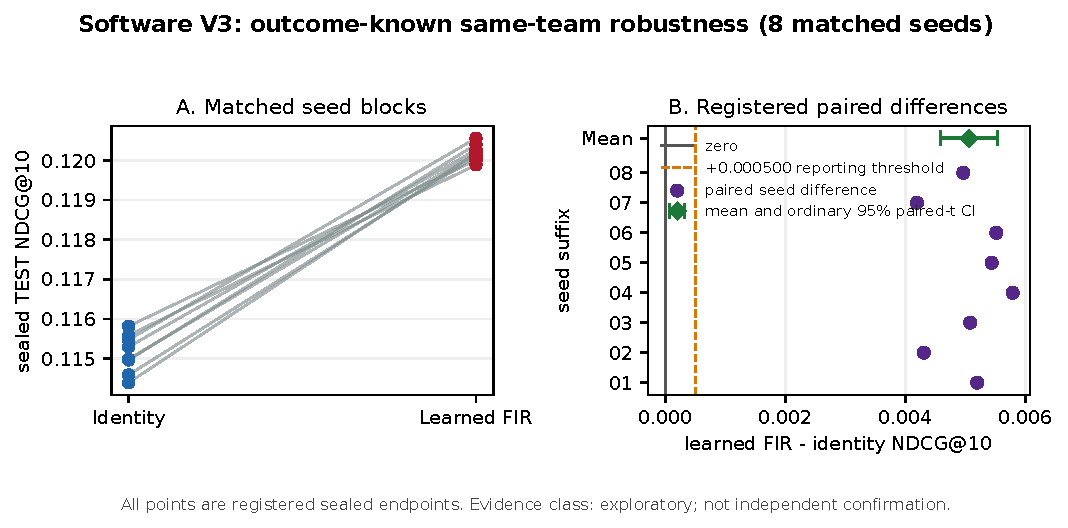
\includegraphics[width=0.96\linewidth]{fig_software_v3_pairs.pdf}
  \Description{Two panels visualize the eight Software V3 matched seed blocks. The left panel connects each identity NDCG at 10 value to its learned-FIR value. The right panel shows all eight learned-minus-identity differences, the zero line, the predeclared plus 0.000500 reporting threshold, and the paired mean with its ordinary 95 percent paired-t confidence interval.}
  \caption{Software V3 registered paired-seed detail. Every matched seed block has higher sealed TEST NDCG@10 under learned FIR than identity; the second panel shows all paired differences, the frozen +0.000500 threshold, and the ordinary paired-t mean and 95\% CI. This is outcome-known same-team robustness, not independent confirmation. Exact values are in \texttt{figures/fig\_software\_v3\_pairs\_data.csv}.}
  \label{fig:software_v3_pairs}
\end{figure}

\clearpage
\section*{S.7 --- Selected-checkpoint FIR diagnostics}

\begin{figure}[h]
  \centering
  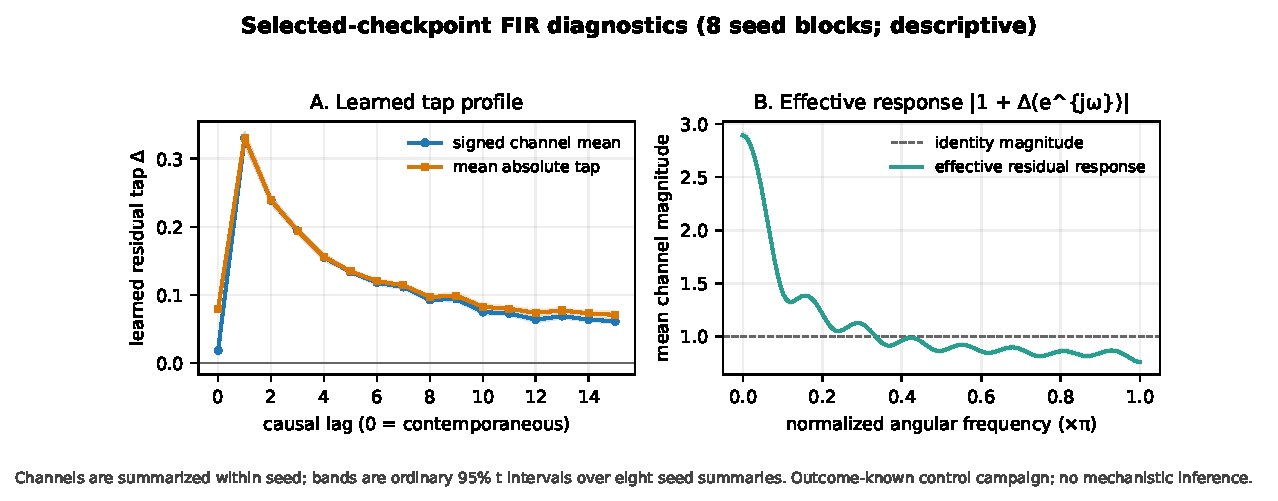
\includegraphics[width=0.96\linewidth]{fig_fir_response.pdf}
  \Description{Two-panel descriptive FIR diagnostic. Panel A plots the
  signed channel-mean residual tap and mean absolute residual tap across
  causal lags 0 through 15, with uncertainty bands over eight seed summaries.
  Panel B plots the magnitude of the effective residual frequency response
  across normalized angular frequency, with an identity-magnitude reference
  at one and an uncertainty band over the same eight seeds.}
  \caption{Learned residual-tap and effective frequency-response summaries from
  the eight released selected checkpoints of the outcome-known active-control
  learned arm. Channels are summarized within each seed; bands are ordinary
  95\% $t$ intervals over the eight seed summaries. Lag 0 is contemporaneous.
  These are descriptive fitted-operator diagnostics, not a mechanism or
  independent-confirmation test; plotted values are released in
  \texttt{figures/fig\_fir\_response\_data.csv}. The effective kernel is the
  residual identity plus the learned $\Delta$ taps.}
  \label{fig:fir-response}
\end{figure}
\endgroup


\bibliographystyle{ACM-Reference-Format}
\bibliography{references}

\end{document}
